\documentclass{beamer}
\usepackage[utf8]{inputenc}
\usepackage{graphicx}
\usetheme{Warsaw}

\title{HLA and Nanopore}
\author{Szilveszter Juhos}
\institute{SciLifeLab}
\date{17. Aug. 2016 }
\begin{document}
\frame{\titlepage}
			  
\begin{frame}
\frametitle{HLA and Nanopore}
\begin{itemize}
	\item we got reads from earlier chemistry (13300 2D reads)
	\item error-prone readings: had a hard time with demultiplexing
	\item we were able to use only ~100 reads for each sample
\end{itemize}

\begin{block}{but most importantly:}
we can have fully phased sequences for the whole HLA-A gene! 
\end{block}
\end{frame}

\begin{frame}
\frametitle{Icing Workflow}
\begin{itemize}
	\item In nexflow (what else), but using other tools like bwa, canu
	\item Demultiplexing and allele selection in python
	\item On github: https://github.com/NationalGenomicsInfrastructure/icing
	\item The name is the icing on the mignon cake: 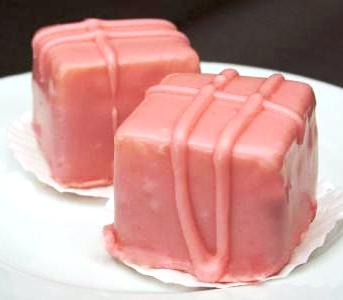
\includegraphics[width=0.3\linewidth]{minyon.jpg}
\end{itemize}
\end{frame}

\begin{frame}
\frametitle{Icing Workflow}
\begin{itemize}
	\item demultiplex pooled input 2D FASTQ
	\item 2D read alignment with BWA to genomic sequences only from IMGT/HLA
	\item select some candidates from the IMGT/HLA database (best matching alleles)
	\item extract reads mappable to these candidates
	\item generate consensus sequences alleles with canu
	\item do the actual HLA typing based on the final consensus sequences and the whole IMGT/HLA database
\end{itemize}
\end{frame}

\begin{frame}
\frametitle{Demultiplexing}
\begin{itemize}
	\item Current indexes are short (6bps), but we have handle sequences (around 25bps)
	\item handle - index - handle = alltogether about 50 bps
	\item using Smith-Waterman to find forward and reverse matching sequences with few mismatches
	\item We hope it will be much better for the new chemistry AND by using longer index sequences as now we 
had to throw away 90\% of our data
\end{itemize}
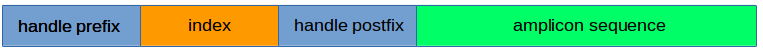
\includegraphics[width=0.9\linewidth]{handle_index.png}
\end{frame}

\begin{frame}
\frametitle{Where we are and what next}
\begin{itemize}
	\item Managed to correctly type the 9 samples from 8 individuals
	\item We really have fully phased FASTA consensuses for HLA-A, as expected
	\item Plan is to do sequencing for HLA-A,B,C and HLA-DRB1 and HLA-DQB1 pooled
	\item Also use new flowcell/chemistry and better indexes, much less DNA
	\item Generating consensuses should be easy.
\end{itemize}
\end{frame}

\end{document}

